\chapter{Implementation and Verification}
\label{sec:implementation}

This section outlines the integration of the new weight update scheme proposed by \citeauthor{jiaRemovalFeedbackLoop2025} into the hardware accelerator implemented by \citeauthor{vorhaugHyperspectralImageCompression2024}. The use of this new weight update scheme results in a compressor that is no longer compliant with the issue 2 standard. Because of this, the CNES decompressor can no longer be used to decompress, and thus verify, the results. No open-source issue 2 compliant decompressors are available, prompting the need for the development of such a tool. Before the changes to the hardware accelerator are presented, the outline for developing an open-source issue 2 decompressor is covered.

\section{Open-source Decompressor}

As shown in section \autoref{sec:compression}, the issue 2 compressor and decompressor have many similarities. This is especially true for the predictor stage, but also applies to the processing of header configuration. To shorten the development time, the verification model written by \citeauthor{vorhaugHyperspectralImageCompression2024} was used as a starting point for the implementation of the decompressor. As opposed to the verification model, the decompressor is not only needed for verification purposes. To successfully integrate the delayed weight updates into the on-board compressor, the decompressor must be able to operate on full scale satellite images. This means that the execution time and memory usage of the program must be kept in mind during development.

\begin{figure}[ht]
	\begin{center}
		
\includegraphics[angle=90, width=0.8\textwidth]{figures/lacrau_cropped.jpg}
	\end{center}
	\caption{Crop of \acrshort{hypso} image used for profiling of the verification model, marked with white, stippled outline.}
	\label{fig:lacrau-cropped}
\end{figure}

To analyse the execution time and memory usage of the verification model, profiling tools were used. These track the \acrshort{CPU} time and memory usage of the program during execution, and the results are usually visualised using a flamegraph. The analysis done here only aims to give a rough overview of the most time and memory consuming sections of the program, and thus only a simple analysis is made. The stippled outline of the \acrshort{hypso} image shown in \autoref{fig:lacrau-cropped} was used as the input for the verification model during profiling. The cropped image has $80$ spectral bands and a spatial size of $70\text{x}150$ samples. The compressor was configured in reduced prediction mode with narrow local sums, using the hybrid encoder and three prediction bands, giving a compression ratio of $2.47$.

The profiling results are summarized in \autoref{tab:profile}, showing the total execution time and memory usage. Results vary depending on the characteristics of the image used, algorithm configuration, and hardware used to run the program. Thus, the numbers shown in the table should only be used as a hint as to the performance of different stages of the calculation. Most notably, the prediction stage occupies $65.2\%$ of the execution time. Additionally, a significant amount of time is spent storing the intermediary results to files. This is because moving data from memory to disk is very slow. The hybrid encoder is responsible for $83.1\%$ of the heap memory allocated by the program. Note that even for such a small image, a rather large chunk of memory (1203MB) is allocated. Based on this analysis, two main approaches to improve the performance of the decompressor are used: a full rewrite of the predictor stage and setting the storing of intermediate results as optional. This targets the two main time consumers of the program, namely the predictor and saving of outputs to disk.

\begin{table}[ht]
	\caption{\acrshort{CPU} time and memory use profile for image compression using verification model.}
	\label{tab:profile}
	\begin{center}
		\begin{tabular}{lrr}
			\hline
			\textbf{Module} & \textbf{CPU Time} & \textbf{Memory Use} \\
			\hline
			Total           & 22.9s             & 1203MB              \\
			Loading         & 0.3\%             & 5.7\%               \\
			Predictor       & 65.2\%            & 11.2\%              \\
			Hybrid encoder  & 16.7\%            & 83.1\%              \\
			Save outputs    & 17.8\%            & N/A                 \\
			\hline
		\end{tabular}
	\end{center}
\end{table}

Python is an interpreted language with dynamic typing. Such programming languages are known to be significantly slower than traditional compiled languages with static typing. Commonly, Python libraries such as Numpy are implemented in compiled languages such as C, C++ or Rust. By use of special libraries and builtin support in the Python language, bindings to the compiled library are created that allow classes and other objects to be used by Python. This combines the simple syntax and fast development times enabled by Python with the high speeds of precompiled libraries. In order to improve the performance of the predictor stage while reusing the encoder and header readers of the old verification model, this work rewrites the predictor stage in C++. By use of the library \textit{pybind11}, bindings are created that allow the new predictor class to be instantiated by the old Python framework. The interface of the new class is identical to that of the old class, while allowing data to be passed between the C++ and Python programs at runtime.

\begin{figure}[ht]
	\begin{center}
		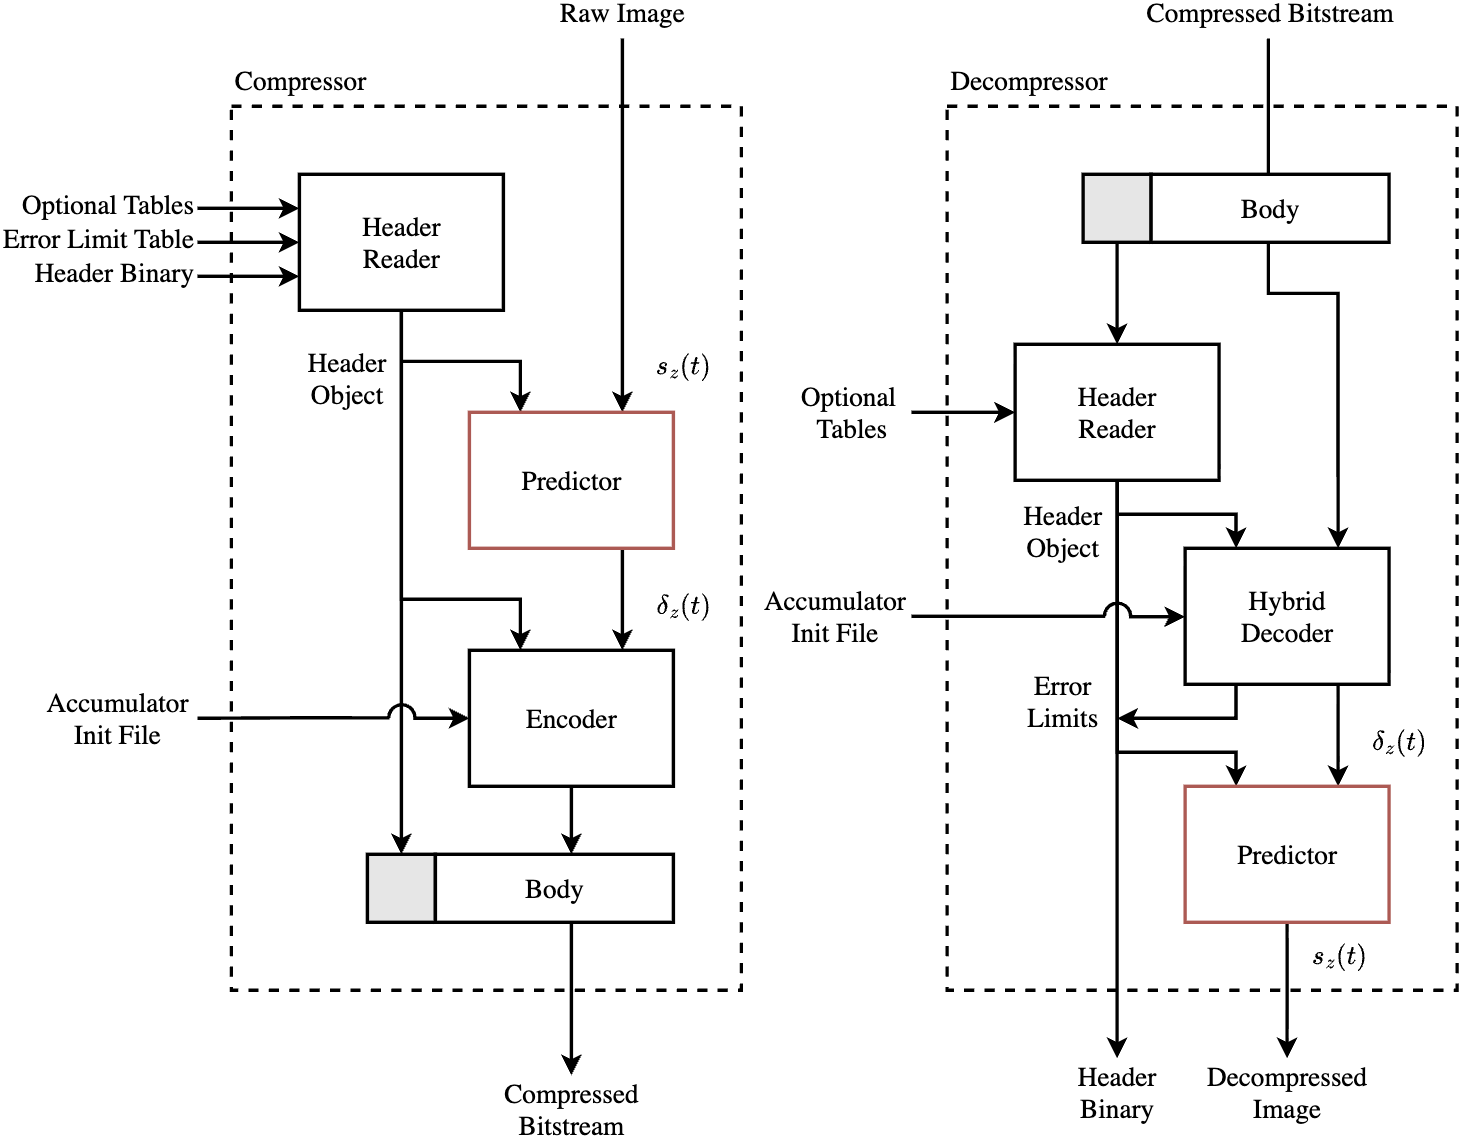
\includegraphics[width=1\textwidth]{figures/verification-model.png}
	\end{center}
	\caption{}
	\label{fig:verification-model}
\end{figure}


% Predictor with compression and decompression implementation in C++. Pybind11, integration with build system. PiP, scikit, Numpy arrays in cpp. Memory ordering and quick access to arrays. Life of allocated memory.
%
% Reconstruction of mapped quantizer indices from compressed bitstream, hybrid encoder.
%
% Header reader used for reading header config from compressed bitstream.
%
% When decoding, also read encoded error limits and set in header class. Output as file in the end.
%
% Note on predictor data types
%
% When storing final, decompressed image make sure to store in correct ordering.
%
% Sampler class.
%
% Construction of verification data: using CNES decompressor with test vector set.
%
% Bitarray module for python.
%
% Rounding bit added to bitstream to allow reconstruction of average estimate model.
%
% Debugging framework, reference file. Debugging flow?

\begin{lstlisting}[
    float=ht,
    caption={Pseudocode for hybrid decoder.},
    label=lst:pseudocode,
    language=Python]
accumulator, active_prefixes = decode_image_tail()
counter                      = get_counter_value(t_max)

for all z and t: # iterate in reverse order
    mapped_quantizer_index[z, t] = decode_sample(z, t)
    if ordering = BI and prediodic_error_limit_updating:
        header.error_limits[z] = decode_error_limts(z)

def decode_sample(z, t): # pops bits from compressed bitstream
    if t = 0: # first sample encoded as is
        mapped_quantizer_index[z, t] = read_D_bit_integer()
    else:
        if accumulator[z, t] * 2^14 >= threshold[0] * counter[t]:
            mapped_quantizer_index[z, t] = decode_high_entropy(z, t)
        else:
            mapped_quantizer_index[z, t] = decode_low_entropy(z, t)

    t_next = t-1
    counter[t_next] = get_counter_value(t_next)

    # update accumulator
    if counter[t_next] = 2^rescaling_counter_size - 1: # rescaling
        rounding_bit = bitstream.pop()
        updated_accumulator = 2 * accumulator[z, t] - 4 * mapped_quantizer_index[z, t] - 1

        if rounding_bit = 0 and updated_accumulator_lsb = 1:
            updated_accumulator += 1 # ensure even
        else if rounding_bit = 1 and updated_accumulator_lsb = 0:
            updated_accumulator += 1 # ensure odd
        accumulator[z, t_next] = updated_accumulator

    else: # normal case
        accumulator[z, t_next] = accumulator[z, t] - 4 * mapped_quantizer_index[z, t]
\end{lstlisting}

\section{Hardware Modifications}

\begin{figure}[ht]
	\begin{center}
		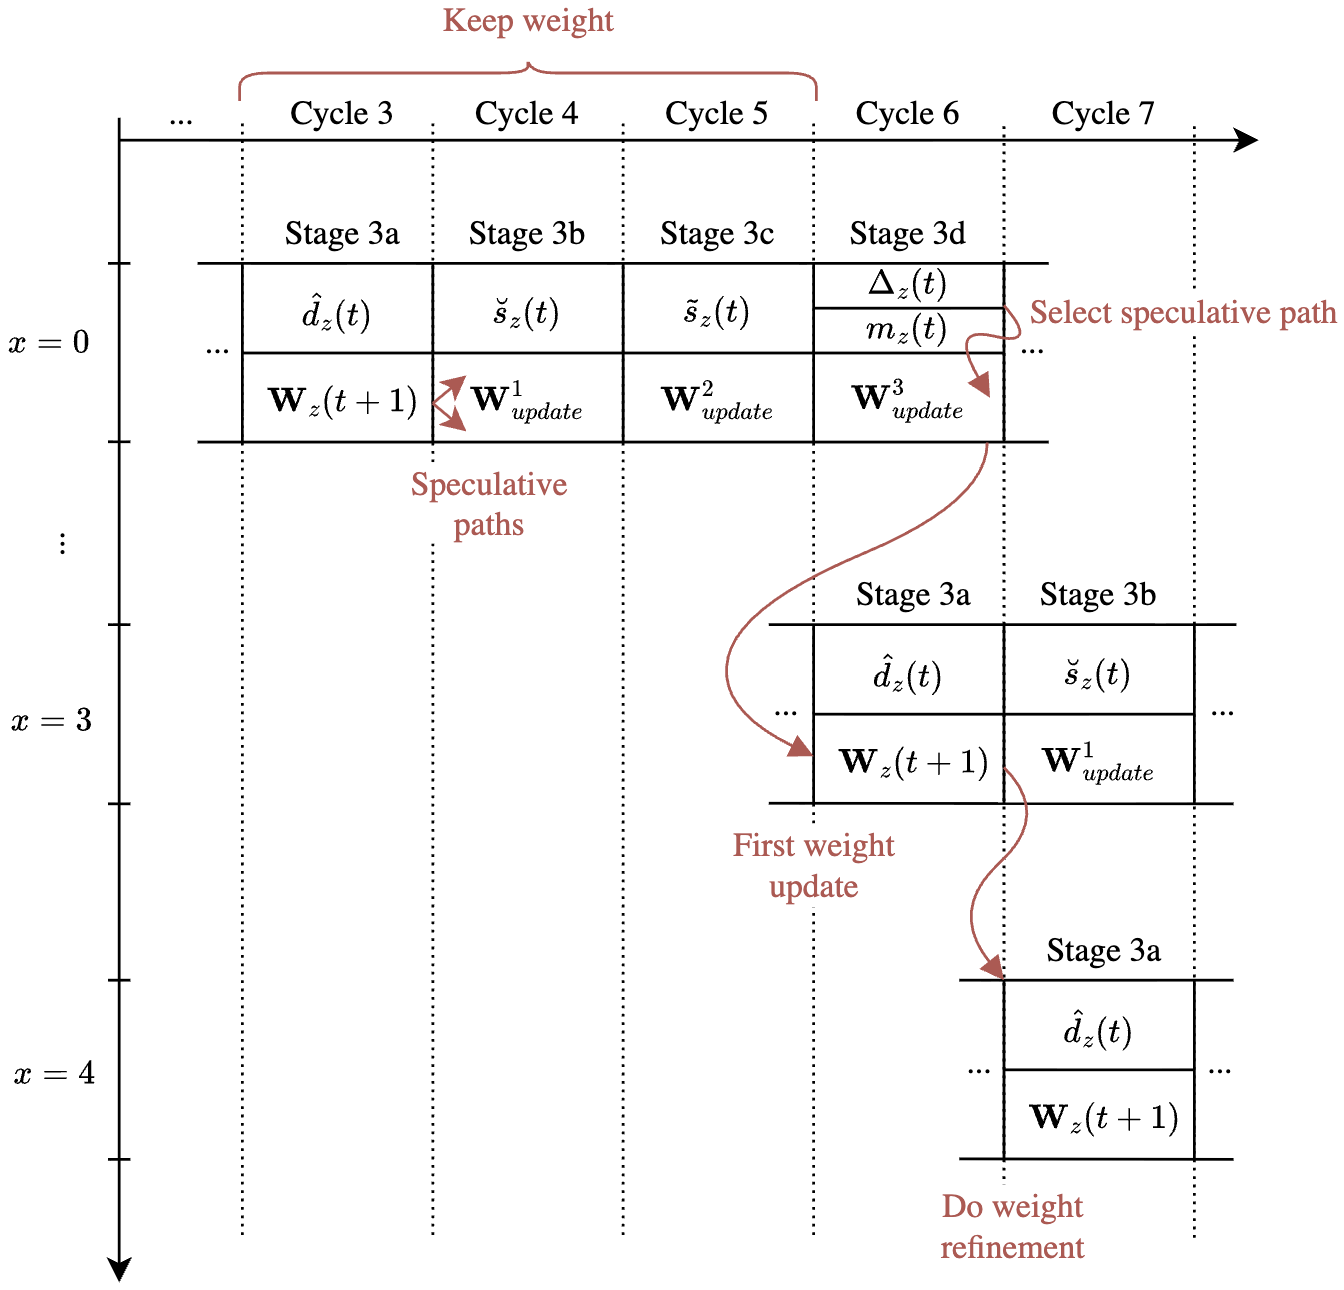
\includegraphics[width=0.85\textwidth]{figures/new-stage3.png}
	\end{center}
	\caption{Proposed pipeline for delayed weight updates.}
	\label{fig:new-stage3}
\end{figure}

\begin{figure}[ht]
	\begin{center}
		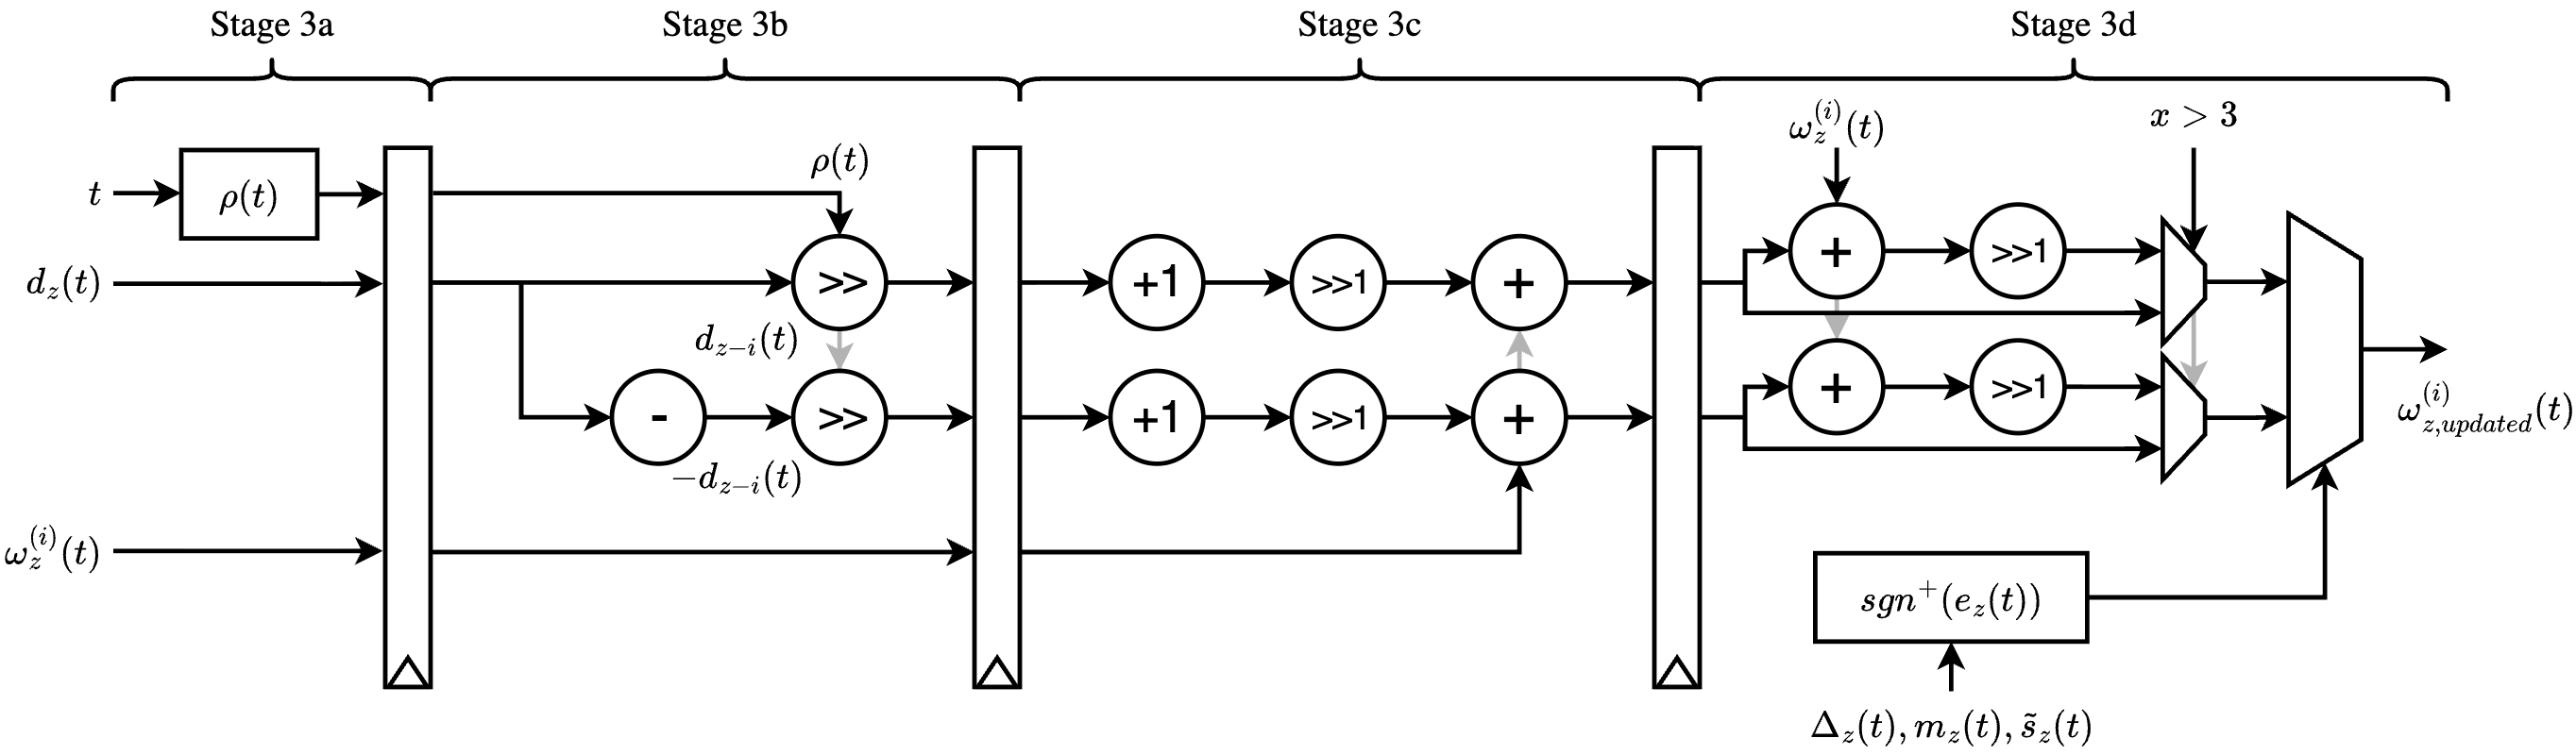
\includegraphics[width=1\textwidth]{figures/weights-pipeline-hw.png}
	\end{center}
	\caption{}
	\label{fig:weights-pipeline-hw}
\end{figure}

\begin{figure}[ht]
	\begin{center}
		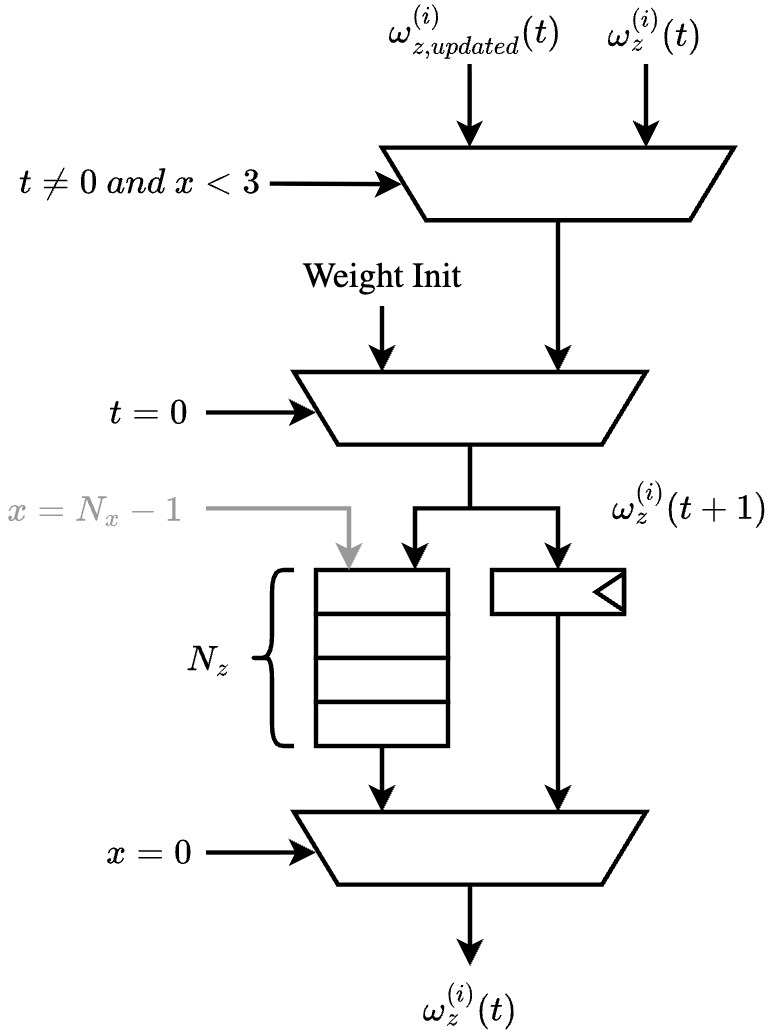
\includegraphics[width=0.45\textwidth]{figures/weights-hw.png}
	\end{center}
	\caption{}
	\label{fig:weights-hw}
\end{figure}

% Analysis of the new critical path after implementation of the new weight update scheme showed that the new path was in the sample representative stage

\begin{figure}[ht]
	\begin{center}
		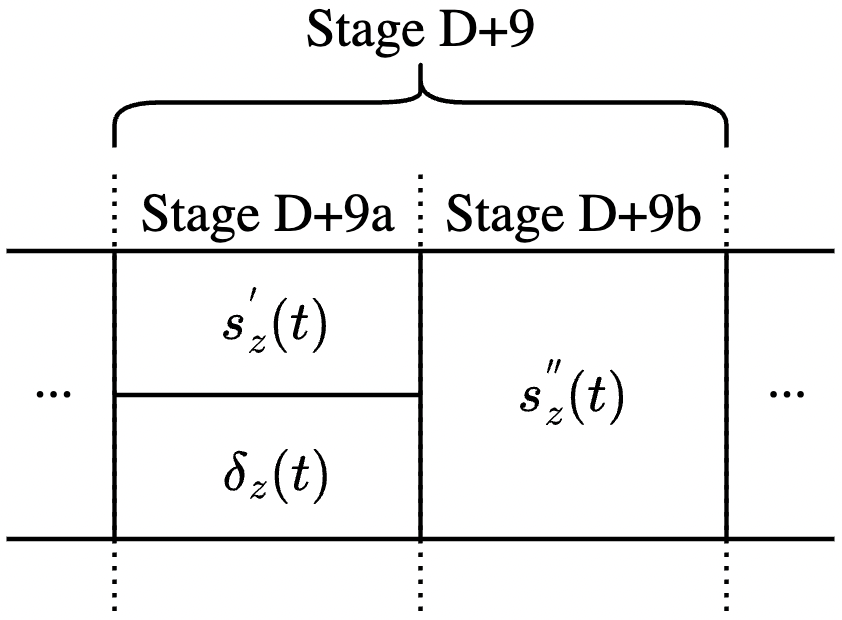
\includegraphics[width=0.3\textwidth]{figures/new-stageD9.png}
	\end{center}
	\caption{Sample representative stage split into two stages $D+9a$ and $D+9b$, reducing the new critical path after splitting the weight update stage.}
	\label{fig:new-stageD9}
\end{figure}

\begin{figure}[ht]
	\begin{center}
		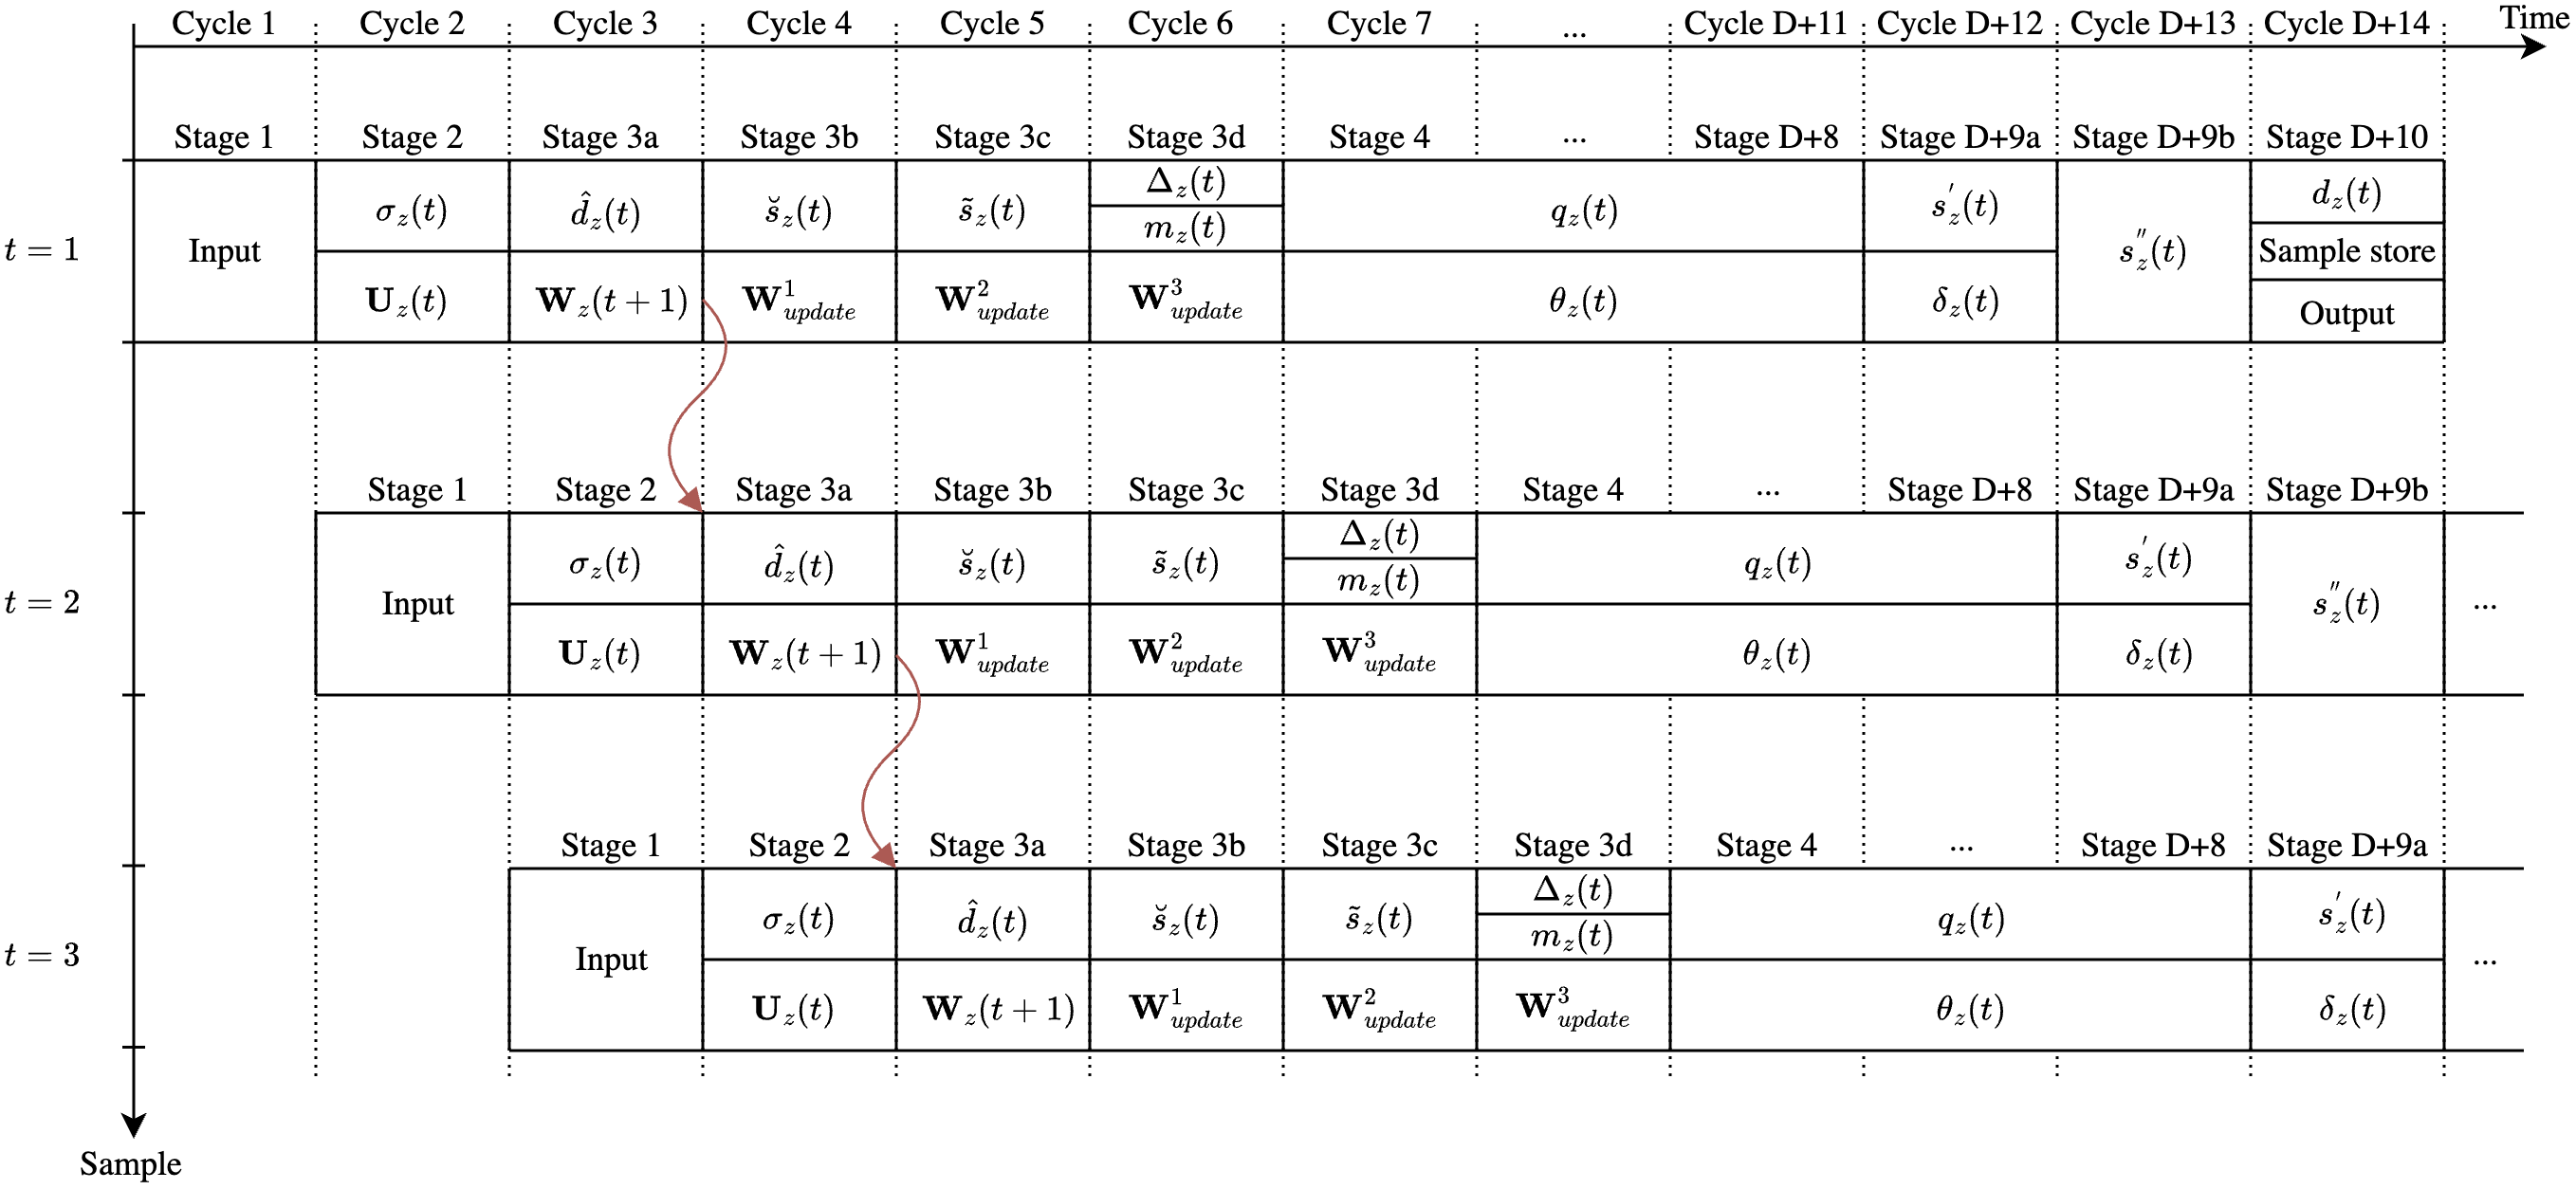
\includegraphics[angle=90, height=1\textheight]{figures/new-pipeline.png}
	\end{center}
	\caption{Proposed pipeline with delayed weight updates allowing splitting stage 3 into four separate stages, 3a to 3d. Additionally, the sample representative calculation in stage $D+9$ is split into two stages $D+9a$ and $D+9b$.}
	\label{fig:new-pipeline}
\end{figure}

\section{Hardware Verification}

\section{Hardware Testing}

\begin{table}[ht]
	\centering
	\caption{Selected predictor and hybrid encoder parameters. Values are selected based on the work by \citeauthor{blanesPerformanceImpactParameter2019}, and are the same as those used by \citeauthor{vorhaugHyperspectralImageCompression2024} \cite{blanesPerformanceImpactParameter2019, vorhaugHyperspectralImageCompression2024}. Table recreated from \cite{vorhaugHyperspectralImageCompression2024}.}
	\label{tab:parameters}
	\begin{tabular}{lcl}
		\toprule
		\textbf{Name}                    & \textbf{Symbol}              & \textbf{Configuration} \\
		\midrule
		Sample type                      &                              & Unsigned               \\
		Dynamic range                    & $D$                          & 16                     \\
		Sample encoding order            &                              & BIL                    \\
		Entropy coder type               &                              & Hybrid coder           \\
		Quantizer method                 &                              & Absolute               \\
		Number of prediction bands       & $P$                          & 3                      \\
		Register size                    & $R$                          & 64                     \\
		Local sum type                   &                              & Narrow column-oriented \\
		Prediction mode                  &                              & Reduced                \\
		Weight component resolution      & $\Omega$                     & 19                     \\
		Weight initialization method     &                              & Default                \\
		Weight update initial parameter  & $\nu_{\min}$                 & $-1$                   \\
		Weight update final parameter    & $\nu_{\max}$                 & $4$                    \\
		Weight update change interval    & $t_{\text{inc}}$             & $2^6$                  \\
		Weight update exponent offsets   & $\zeta_z^{(i)}, \zeta_z^{*}$ & $0$                    \\
		Periodic error limit update      &                              & Disabled               \\
		Band-varying absolute limits     &                              & Disabled               \\
		Absolute error limit             & $a_z$                        & \emph{Varied}          \\
		Band-varying relative limits     &                              & Disabled               \\
		Relative error limit             & $r_z$                        & $0$                    \\
		Sample representative resolution & $\Theta$                     & $3$                    \\
		Sample representative offset     & $\psi_z$                     & $7$                    \\
		Band-varying offset              &                              & Disabled               \\
		Sample representative damping    & $\theta_z$                   & $3$                    \\
		Band-varying damping             &                              & Disabled               \\
		Unary length limit               & $U_{\max}$                   & $18$                   \\
		Rescaling counter size           & $\gamma^{*}$                 & $6$                    \\
		Initial count exponent           & $\gamma_0$                   & $1$                    \\
		Accumulator initialization value & $\tilde{\Sigma}_z(0)$        & $4 \cdot 2^{\gamma_0}$ \\
		\bottomrule
	\end{tabular}
\end{table}
